\documentclass[10pt,conference]{IEEEtran}

\if CLASSINFO
	\usepackage[pdftex]{graphicx}
	%\graphicspath{{./figs/}}
	\DeclareGraphicsExtensions{.pdf,.jpeg,.png}
\else
	\usepackage[dvips]{graphicx}
	%\graphicspath{{./figs/}}
	\DeclareGraphicsExtensions{.eps}
\fi

\usepackage[cmex10]{amsmath}
\usepackage[tight,footnotesize]{subfigure}

\usepackage{xcolor}
\usepackage[lined,ruled]{algorithm2e}

\usepackage[latin1]{inputenc}
\usepackage{tikz}
\usetikzlibrary{shapes}
\usetikzlibrary{arrows}

\usepackage[]{algorithm2e}
\usepackage{pdfpages} 

\newtheorem{property}{Property}
\newtheorem{proposition}{Proposition}
\newtheorem{theorem}{Theorem}
\newtheorem{conjecture}{Conjecture}
\newtheorem{question}{Question}
\newtheorem{definition}{Definition}
\newtheorem{corollary}{Corollary}

\makeatletter
\pgfdeclareshape{datastore}{
  \inheritsavedanchors[from=rectangle]
  \inheritanchorborder[from=rectangle]
  \inheritanchor[from=rectangle]{center}
  \inheritanchor[from=rectangle]{base}
  \inheritanchor[from=rectangle]{north}
  \inheritanchor[from=rectangle]{north east}
  \inheritanchor[from=rectangle]{east}
  \inheritanchor[from=rectangle]{south east}
  \inheritanchor[from=rectangle]{south}
  \inheritanchor[from=rectangle]{south west}
  \inheritanchor[from=rectangle]{west}
  \inheritanchor[from=rectangle]{north west}
  \backgroundpath{
    %  store lower right in xa/ya and upper right in xb/yb
    \southwest \pgf@xa=\pgf@x \pgf@ya=\pgf@y
    \northeast \pgf@xb=\pgf@x \pgf@yb=\pgf@y
    \pgfpathmoveto{\pgfpoint{\pgf@xa}{\pgf@ya}}
    \pgfpathlineto{\pgfpoint{\pgf@xb}{\pgf@ya}}
    \pgfpathmoveto{\pgfpoint{\pgf@xa}{\pgf@yb}}
    \pgfpathlineto{\pgfpoint{\pgf@xb}{\pgf@yb}}
 }
}
\makeatother

\newcommand{\riham}[1]{{\color{red}{#1}}}
\newcommand{\james}[1]{{\color{blue}{#1}}}


\begin{document}

\title{CS-336 Airport Management Database}
\author{
\IEEEauthorblockN{Harsha Bodapati}
\IEEEauthorblockA{Rutgers University\\ Piscataway, NJ, USA\\
}
\and
\IEEEauthorblockN{Jiahui Chen}
\IEEEauthorblockA{Rutgers University\\
Piscataway, NJ, USA\\
}
\and
\IEEEauthorblockN{Parth Shorey}
\IEEEauthorblockA{Rutgers University\\
Piscataway, NJ, USA\\
}
%\and
%\IEEEauthorblockN{Third group member}
%\IEEEauthorblockA{Rutgers University\\
%\Piscataway, NJ, USA\\
%Email: Third_group_member@scarletmail.rutgers.edu}
}


                                                                                                                                                                                                                                                                               \maketitle


\begin{abstract}
\textnormal{
The purpose of this project is to create a database model, which will consist of multiple views, to help manage information for an airport. 
The database will have back end that can handle scalability and provides a rigid front end. The backend will be written mostly in Standard Query Language (SQL) and
PHP. The front end will be a kind of user interface made using a combination of HTML and XML.
}
\end{abstract}
%\onecolumn \maketitle \normalsize \vfill

\IEEEpeerreviewmaketitle
 %%%%%%%%%%%%%%%%%%%%%%%%%%%%%%%%%%%%%%%%%%%%%%%%%%%%%%%%%%%%%%%%%%%%%%%%%%%%%%%%%%%%%%%%%%%%%%%%%%%%%%%%%
\section{Project Description}\label{sec:1. Project Description}
%\input{introduction.tex}
%%%%%%%%%%%%%%%%%%%%%%%%%%%%%%%%%%%%%%%%%%%%%%%%%%%%%%%%%%%%%%%%%%%%%%%%%%%%%%%%%%%%%%%%%%%%%%%%%%%%%%%%%
\textnormal{
This database has the information on administrators, staff members, flight attendants, and 
passengers consisting of aspects such as contact info, salary, experience, name of aircraft, and location of airport. Regular users such as passengers can view information on timings and location for their flight. Flight attendants can interact with this data to view the information about the passengers. Also, this repository will maintain the admins who have the most access to information about passengers and managing the attendants. This database is useful to people because it can help them get in touch with one another simply and organize the flight properly in order to reach the destination safely and efficiently. 
}
\subsection{Stage1 - The Requirement Gathering Stage. }\label{sec:1.	Requirement Gathering Stage. }
%%%%%%%%%%%%%%%%%%%%%%%%%%%%%%%%%%%%%%%%%%%%%%%%%%%%%%%%%%%%%%%%%%%%%%%%%%%%%%%%%%%%%%%%%%%%%%%%%%%%%%%%%%

User 1- Administrators: have the highest access right. An administrator has access to:
\begin{itemize}
\item Staff Member\_data(ID, name, contact info, salary, experience etc.)
\end{itemize}

\begin{itemize}
\item Flight attendants\_data(ID, name, contact info, salary, experience etc.)
\end{itemize}

\begin{itemize}
\item Passengers\_data(ID, name, contact info, VIP or not etc.)
\end{itemize}

\begin{itemize}
\item Flights\_data(schedule, flight crew assigned, nonstop flight or not, departure airport, arrival airport etc.)
\end{itemize}

\begin{itemize}
\item Aircrafts\_data(ID, name, model, year made, carrying capacity etc.)
\end{itemize}

\begin{itemize}
\item Airports\_data(name, location etc.)
\end{itemize}






User 2- Staff Member: have the second highest level of access right. A staff member has access to:
\begin{itemize}
\item Passengers\_data(ID, name, contact info, VIP or not etc.)(FULL)
\end{itemize}

\begin{itemize}
\item Flights\_data(schedule, flight crew assigned, nonstop flight or not, departure airport, arrival airport etc.)
\end{itemize}

\begin{itemize}
\item Aircrafts\_data(ID, name, model, year made, carrying capacity etc.)
\end{itemize}

\begin{itemize}
\item Airports\_data(name, location etc.)
\end{itemize}




User 3- Flight attendants/Captain: have the third highest level of access right. A Flight attendant has access to:
\begin{itemize}
\item Flights\_data(schedule, flight crew assigned, nonstop flight or not, departure airport, arrival airport etc.)
\end{itemize}

\begin{itemize}
\item Passengers\_data(ID, name, contact info, VIP or not etc.)(LIMITED)
\end{itemize}

\begin{itemize}
\item Aircrafts\_data(ID, name, model, year made, carrying capacity etc.)
\end{itemize}

\begin{itemize}
\item Airports\_data(name, location etc.)
\end{itemize}




User 4- Passengers: have the lowest access right. A passenger has access to:
\begin{itemize}
\item Flights\_data(schedule, flight crew assigned, nonstop flight or not, departure airport, arrival airport etc.)
\end{itemize}

\begin{itemize}
\item Airports\_data(name, location etc.)
\end{itemize}\vspace{5mm}

Scenario 1 for Passengers:
John went to a conference meeting held in San Francisco. The flight John took is operated by Delta Airline which departures from Newark international airport at 10:00pm and arrives at San Francisco international airport at estimated local time 8:00am. The flight has one stop at Dallas international airport. John arrived at the airport two hours before departure; he typed flight number (INTEGER data type) on Delta Airline's mobile app and received the information about the flight: departures at terminal A (CHAR data type) into the system. The boarding pass successfully printed out. Then Johns luggage was scaled and measured (DOUBLE data type). It didn't exceed the limitation and successfully checked in.\vspace{5mm}\\System data input: flight number\\
Input data types: CHAR data type\\
System data output: flight number, terminal number\\
Output data types: CHAR data type, INTEGER data type

\vspace{5mm}
Scenario 2 for Passengers:
While sitting in the waiting area, John found that there is a 30 percent discount on seats upgrading today. He decided to upgrade his seat to business class. John went up to a staff member and told her about it. Staff Nancy checked Johns boarding pass and ID, and entered the ID number (CHAR data type) into the system. After confirming Johns identity, Nancy showed John available seats for upgrading. And John picked seat 3A by the window. Nancy then entered the new seat no. (CHAR data type) into the system and printed out a new boarding pass for John. Having his new boarding pass scanned, John boarded the plane successfully and started his trip to San Francisco. \vspace{5mm}\\System data input: ID number
\\
Input data types: CHAR data type\\
System data output: seat number\\
Output data types: CHAR data type

\vspace{5mm}
Scenario 1 for Admin:
The admin will have access to all information in the database. This will allow the admin to control the way other users view the data as well. One important scenario will be the organization of captains and flight attendants for every flight, and whether or not it is feasible to have them on a particular flight. Because the administrator can access all entities within the database, they can add or delete certain tuples that pertain to the information regarding the captains and flight attendants on a flight. They can do this by selecting the ID of the employees on the plane, and then manipulating their permissions to whatever is feasible. It allows the admin to assign more experienced captains to larger and/or longer flights. This scenario will require the admin to view all information regarding flights, and make a selection of the relevant attributes to organize the data.
So if an admin sees that there is flight going U.S. to Brazil, and Captain and Co-Pilot of that flight have relatively low experience in flying international flights, the admin can look through a table of all captains at that particular airport and select them according to their experience rating (CHAR data type), which in this case would pertain to their ability at flying an international flight.
 \vspace{5mm}\\System data input: flight number, captain(pilot) experience
\\
Input data types: CHAR data type, INTEGER data type\\
System data output: captain(pilot experience) \\
Output data types: INTEGER data type




\vspace{5mm}
Scenario 2 for Admin:
The full access given to the admin comes most in handy during an emergency: if there is an emergency landing caused by a medical emergency or a forced landing due to inclement weather, then the admin will have to designate emergency landing area for the incoming planes and make sure all other planes at the airport are not put in the way of harm. 
The first thing would be for the admin to look up contact info for the plane or captain (both CHAR data types). The next step would be to select of all departing flights (STRING type), arriving after a certain date/time (DATE data type) and ground all those flights by changing their status to delayed (STRING data type). This will allow the the admin to process the incoming emergency flight without any extra obstacles.  \vspace{5mm}\\System data input: captain/plane contact info, date/time, flight statuses
\\
Input data types: CHAR data type, DATE data type, STRING data type
\\
System data output: send information to emergency flight, date/time\\
Output data types: CHAR data type, DATE data type



\vspace{5mm}
Scenario 1 for Flight Attendant:
The flight attendant view will give access to information regarding passenger information, plane information and flight information. It will also access to some things relating to the captain of the plane, in terms of what their rank, their preferences in food, and how to communicate with them. 
The flight attendants will also need to have access for passengers and their seating arrangement. For example, if a passenger says they have been given the wrong meal, the flight attendant can look up this information using the table for passengers and look up the attribute regarding passenger meals (CHAR data type) to check whether or not the correct meal has been given to the complaining passenger. \vspace{5mm}\\System data input: passenger meal
\\
Input data types: CHAR data type\\
System data output: passenger meal check\\
Output data types: CHAR data type




\vspace{5mm}
Scenario 2 for Flight Attendant:
There might be an scenario where the flight attendant has to accommodate a passenger due to some emergency medical condition. This might require the flight attendant to access flight data to check if there is extra space, which can be done by looking up the attribute that shows the number of seats on a plane (INTEGER data type) and number of passengers on the flight (INTEGER data type) and then comparing those using a relation. \vspace{5mm}\\System data input: number of seats on plane
\\
Input data types: INTEGER data type\\
System data output: difference between total seats and passengers on plane 
\\
Output data types: both INTEGER data type, as well as the output




\vspace{5mm}
Scenario 1 for Staff Member:
The first scenario will be deciding how passengers are seated, in relation to where they are traveling, with whom they are traveling with, and if all the passengers will be distributed in the plane equally. This will also affect the number of flight attendants assigned to a flight, because the more passengers, the more flight attendants.
	If there are two flights going to India, back-to-back, and the first one of them is canceled, the admin might take a decision in which he will add some of the people in the first flight to the second flight. This will mean that the admin will have to add more flight attendants.
 \vspace{5mm}\\System data input: flight number
\\
Input data types: INTEGER data type\\
System data output: (new)flight number, time, gate number\\
Output data types: INTEGER data type, TIME data type, CHAR data type



\vspace{5mm}
Scenario 2 for Staff Member:
After a 5-hours flight, John landed in Dallas international airport with a layover for 45 minutes. John took his carry-on bag and walked to the boarding gate for his next flight from Dallas to San Francisco. At the gate, John was informed that his flight was delayed due to aircraft maintenance issues and he need to take a different flight. John was upset and asked airline staff for help. Staff Dave asked for Johns original flight No. (INTEGER data type) and then entered it into the system. In a minute, John received new flight info on his mobile app that flight no. 3522 (INTEGER data type) now departures at 5:00AM (TIME data type) at the gate G21(CHAR data type). Luckily, the new flight was just delayed for one hour and John earned 1000 miles mileage points (INTEGER data type) as a compensatory from the airline company. \vspace{5mm}\\System data input: flight number
\\
Input data types: INTEGER data type\\
System data output: (new)flight number, time, gate number\\
Output data types: INTEGER data type, TIME data type, CHAR data type



\subsection{Stage2 - The Design Stage. }\label{sec: 2:The Design Stage.}
%%%%%%%%%%%%%%%%%%%%%%%%%%%%%%%%%%%%%%%%%%%%%%%%%%%%%%%%%%%%%%%%%%%%%%%%%%%%%%%%%%%%%%%%%%%%%%%%%%%%%%%%%%




\begin{itemize} \item{Specification of each relation and its entities plus attributes} \end{itemize}


\textnormal{The first entity is Flight Attendant. The attributes for this entity consists of contact info, flight attendant ID (which is the key), name, and salary. The second entity is Flight and the attributes associated with it are flight number(key), schedule, terminal, seat, departure of the airport, arrival of the airport, and if it is direct or non-stop flight. The third entity is Plane(Aircraft) which contains the attributes of the year it was made, its plane id(key), its model name, and how many people it can hold (capacity). The fourth entity is Passenger which consists of the attributes passenger ID, name, contact info, and whether that passenger is VIP or not. The fifth entity is staff member which has the attributes staff ID(key), their names, contact info, how much experience they have, and salary. The sixth entity is Captain. The attributes for this entity are experience, contact info, captain ID (which is the key), name, and salary.The seventh entity is Employee with primary key attribute employee ID.} 

\textnormal{The four entities: captain, flight attendant, staff member and employee have a IS-A relation. A captain, a flight attendant or a staff member is an employee. The Work with relation is a unary relation, meaning that a flight attendant works with another flight attendant. The On relation connects three entities: captain, flight and plane. It is a ternary relation which shows that a captain flies a flight on a plane. The Work on relation connects flight attendant entity and flight entity. It has an at most one constrain that a flight attendant can work on at most one flight at one time. Entity Flight has an exactly one constraint which is that one flight can only be on exactly one plane. The relation that connects passenger and staff member is SERVES with at least one constraint. This means that every staff member serves at least one passenger. Also there is an aggregation relationship between Passenger entity and Flight, Plane entities.}


\vspace{5mm}

\begin{itemize} \item{Descriptions relating ER part (relation) to one or more user scenarios} \end{itemize}

\textnormal{Description relating to ER part for Scenario 1 for Passengers: Gives Passenger(view) access to all the information of the flight that is called using a query according to the flight number.      For example,  SELECT F.terminal  FROM  flight F   WHERE F=fid = " "}


\textnormal{Description relating to ER part for Scenario 2 for Passengers: Gives staff member access to all the information of the flight if passenger wants to upgrade his seat that is called using a query according to the confirmation of his ID number and availability of the seat.}


\textnormal{Description for Scenario 1 for Admin: Gives Admin(view) access to all the information of the flight in order to organize it properly that is called using a query according to the flight number and captain(pilot experience).}


\textnormal{Description for Scenario 2 for Admin: Gives Admin(view) access to all the statuses of the flight, contact info about the captain and plane, and date/time in order to be ready for any emergencies that may come up. For example, switch the status of a plane to delayed if inclement weather arises according to the plane info and flight status.}


\textnormal{Description for Scenario 1 for Flight Attendant: Gives Flight Attendant(view) access to information regarding passenger information,
plane and flight information, aspects relating to the captain of the plane like his/her rank, and food preferences. So the attendant can see this information for a passenger and ensure they are getting the correct meal.}


\textnormal{Description for Scenario 2 for Flight Attendant: Gives Flight Attendant(view) access to data of the flight regarding seats in order to accommodate passengers needing a ticket very quickly and it is called using a query according to the number of seats on the plane.}


\textnormal{Description for Scenario 1 for Staff Member: Gives staff member(view) access to all the information of the flights in order to see if passengers and flight attendants are distributed correctly on a flight. For example, if there are two flights going back to back to a destination, then a flight is canceled, a staff member can ensure that passengers move to the other flight and add more attendants to regulate that flight according to the flight number. }

\textnormal{Description for Scenario 1 for Staff Member: Gives staff member(view) access to all the information of the flights in order to see if passengers and flight attendants are distributed correctly on a flight. For example, if there are two flights going back to back to a destination, then a flight is canceled, a staff member can ensure that passengers move to the other flight and add more attendants to regulate that flight according to the flight number. }




\textnormal{Description for Scenario 2 for Staff Member: Gives staff member(view) access to all the information of the flights in order to see the timings of passengers flight in order to provide a better option to board a different flight earlier or later. For example, if a person's flight is delayed 3 hours and there is another one at 5 am that is available, that passenger can board that plane and receive compensation for 1000 mileage points to continue their service with us, and this is all based according to their flight number.}


\begin{figure}
\centering
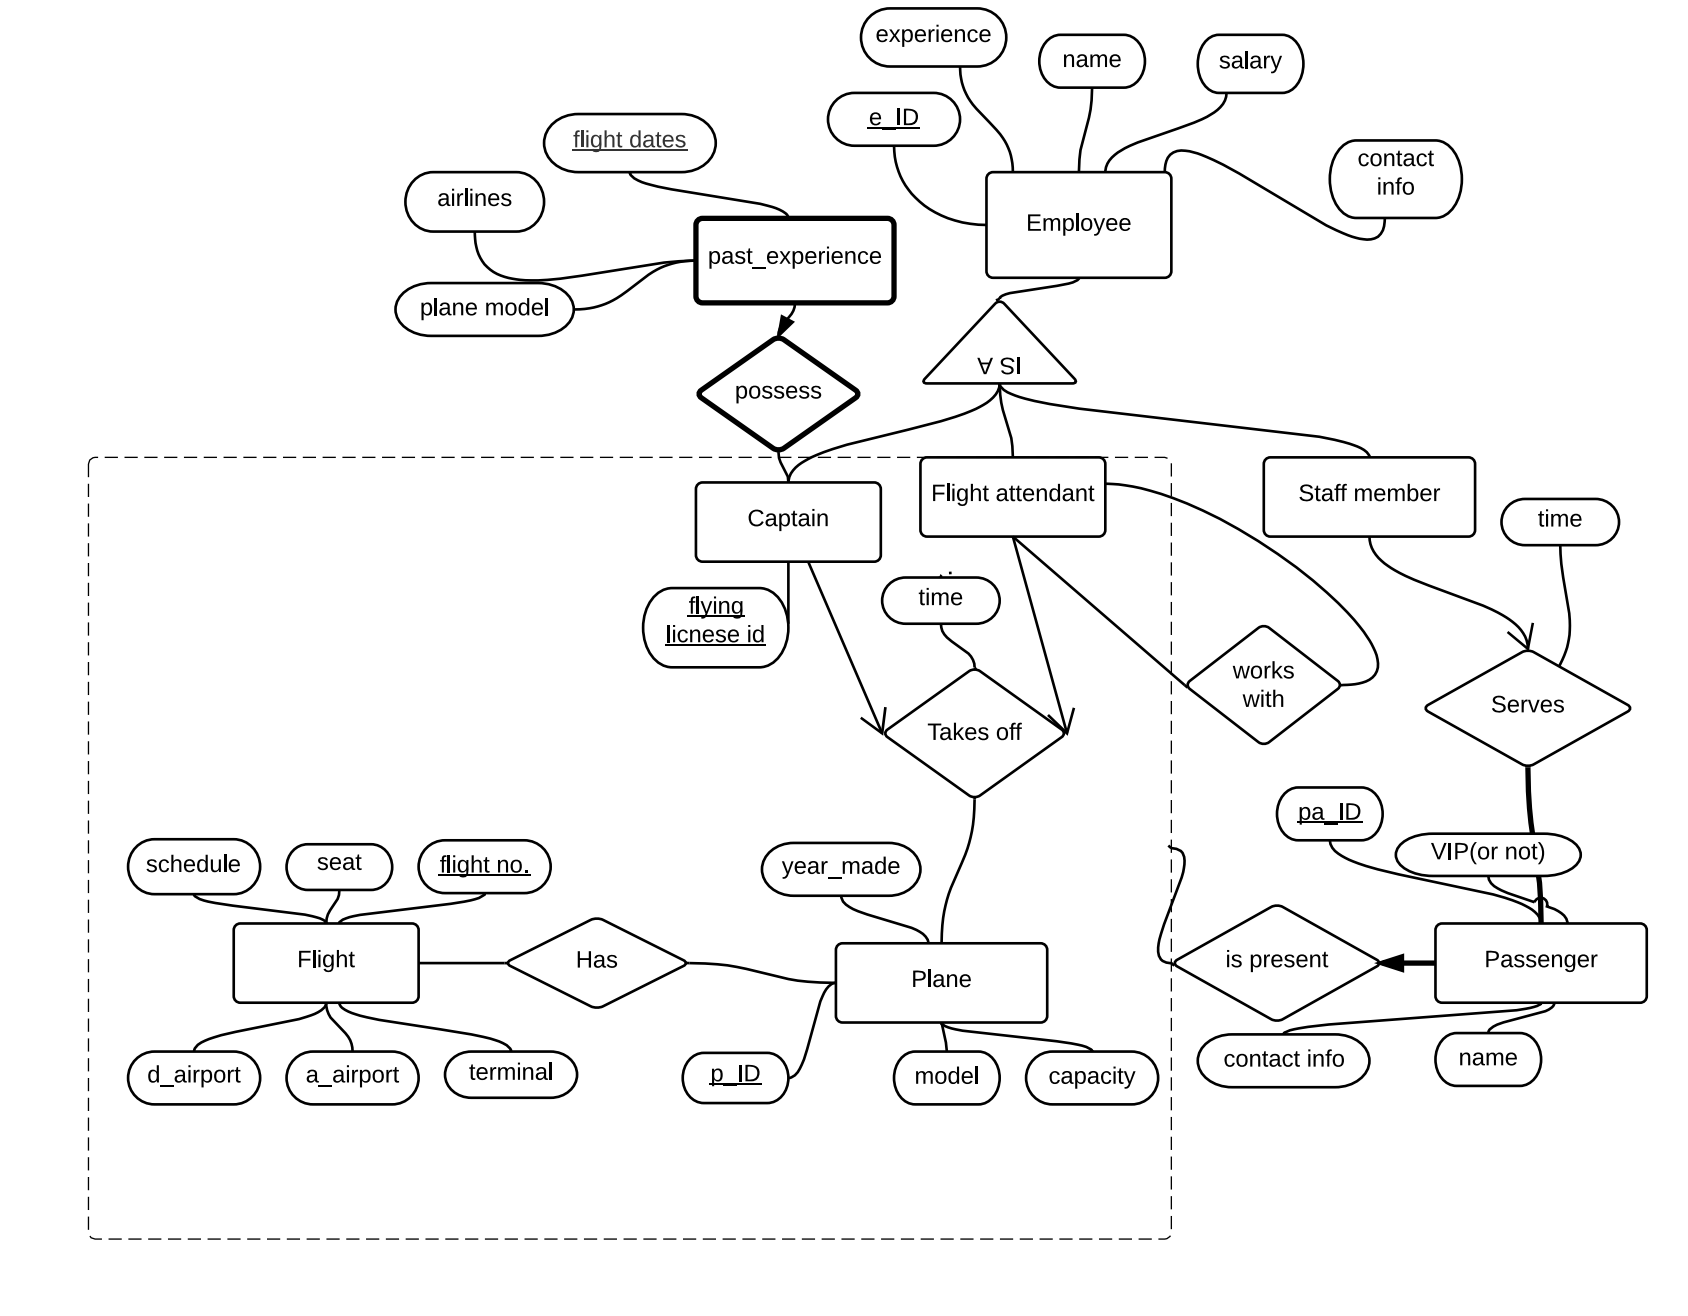
\includegraphics[width=.50\textwidth]{final_icloud_chart.png}
\end{figure}



\vspace{5mm}

\begin{itemize} \item{Brief textual description of the ER diagram(on next page)} \end{itemize}
\textnormal{The ER diagram allows one to visualize the relations we initially described in the scenarios from stage 1; it gives a user a display of how the entities are connected and how manipulating their instantiation would affect other entities in the relation. It allows an understanding of how the views are going to be organized- the ER diagram represents a multi-set of the entire diagram, and the view we intend to create in the future will be a subset of the multi-set.}



\vspace{7mm}


\begin{itemize} \item{
Description and justification of the defined integrity constraints} \end{itemize}

\textnormal{At least one integrity constraint:every staff member serves at least one passenger.}

\textnormal{At most one integrity constraint:a flight attendant can work on at most one flight at one time.}

\textnormal{Exactly one integrity constraint:one flight can only be on exactly one plane.}

\vspace{3mm}
\textnormal{For the Flight attendant entity, the primary key is fa id(flight attendant id) because it uniquely distinguishes each one of them. Also, the domain integrity for each attribute is experience(CHAR), contact info(INTEGER), salary(INTEGER), name(CHAR), and faID(INTEGER). Also, every flight attendant can work on at most one flight. You cannot have a flight attendent assigned to multiple flights, as this would create flights that have missing flight attendents.}
\vspace{3mm}

\textnormal{For the Captain entity, the primary key is cID(Captain ID) because it uniquely distinguishes each one of them. The domain integrity for each attribute is experience(CHAR), contact info(INTEGER), salary(INTEGER), name(CHAR), and cID(INTEGER).}
\vspace{3mm}

\textnormal{For the Flight entity, the key is flight number.Flight number uniquely distinguishes the numbers of the flights in order for the passengers to easily board it. Also, the domain integrity for each attribute is seat(INTEGER), terminal(CHAR), flight number(INTEGER), schedule(CHAR), departure of airport(CHAR), arrival of airport(CHAR), and non stop(CHAR).}
\vspace{3mm}

\textnormal{For the Plane(Aircraft) entity, the primary key is pID (plane ID) because it uniquely distinguishes each aircraft. For example, whether it is Continental, Boeing, or Air India. Also, the domain integrity for each attribute is year made(INTEGER), pID (INTEGER), model name(CHAR), and capacity(INTEGER).}
\vspace{3mm}

\textnormal{For the Employee entity, the primary key is eID(employee ID).It has an IS-A relation with captain entity, flight attendant entity and staff member entity.}
\vspace{3mm}

\textnormal{For the Passenger entity, the primary key is paID (passenger ID) because it uniquely distinguishes each passenger in order for flight attendants and staff members to look them up by their attributes and serve them properly...etc. Also, the domain integrity for each attribute is paID(INTEGER), name(CHAR), contact info(INTEGER), and (not)VIP(CHAR).}
\vspace{3mm}

\textnormal{For the Staff Member entity, the primary key is sID (staff ID) because it uniquely distinguishes each staff member by their certain attributes like name, experience, and salary. For example, if a staff member has more experience, then that particular one will have more salary. Also, the domain integrity for each attribute is sID(INTEGER), name(CHAR), contact info(INTEGER), experience(CHAR), salary(INTEGER). Every staff member services at least one passenger, which creates a constraint for the relationship between passengers and staff member.}

\textnormal{For the past experience entity, the primary key is flight dates and flying license id(note this is a weak entity) because it uniquely distinguishes each pilots identity. Also, the domain integrity for each attribute is flying license id, plane model(CHAR), airlines(CHAR), flight dates(CHAR).}

\begin{itemize} \item{
ER DIagram on top left of page 4, You can zoom in on the image.} \end{itemize}



\vspace{150mm}


\begin{itemize} \item{
Example of Aggregation- There is an AGGREGATION containing the captain, flight attendant, takes off relation, Plane, and Flight.  This represents that passenger has to be present in plane as it takes off with the captain and the flight attendant. The two weak entities going to the strong entity, basically they are a shadow of the "strong" entity which is Plane and there is no flight without Plane taking off and passenger present in it. In everyday life, without the captain, the plane cannot fly and without the FA, it cannot take off in order to help others in the plane. This is a higher-level entity. In terms of SQL, the cid references the captain, faid references flight attendant...etc} \end{itemize}


\begin{figure}
\centering
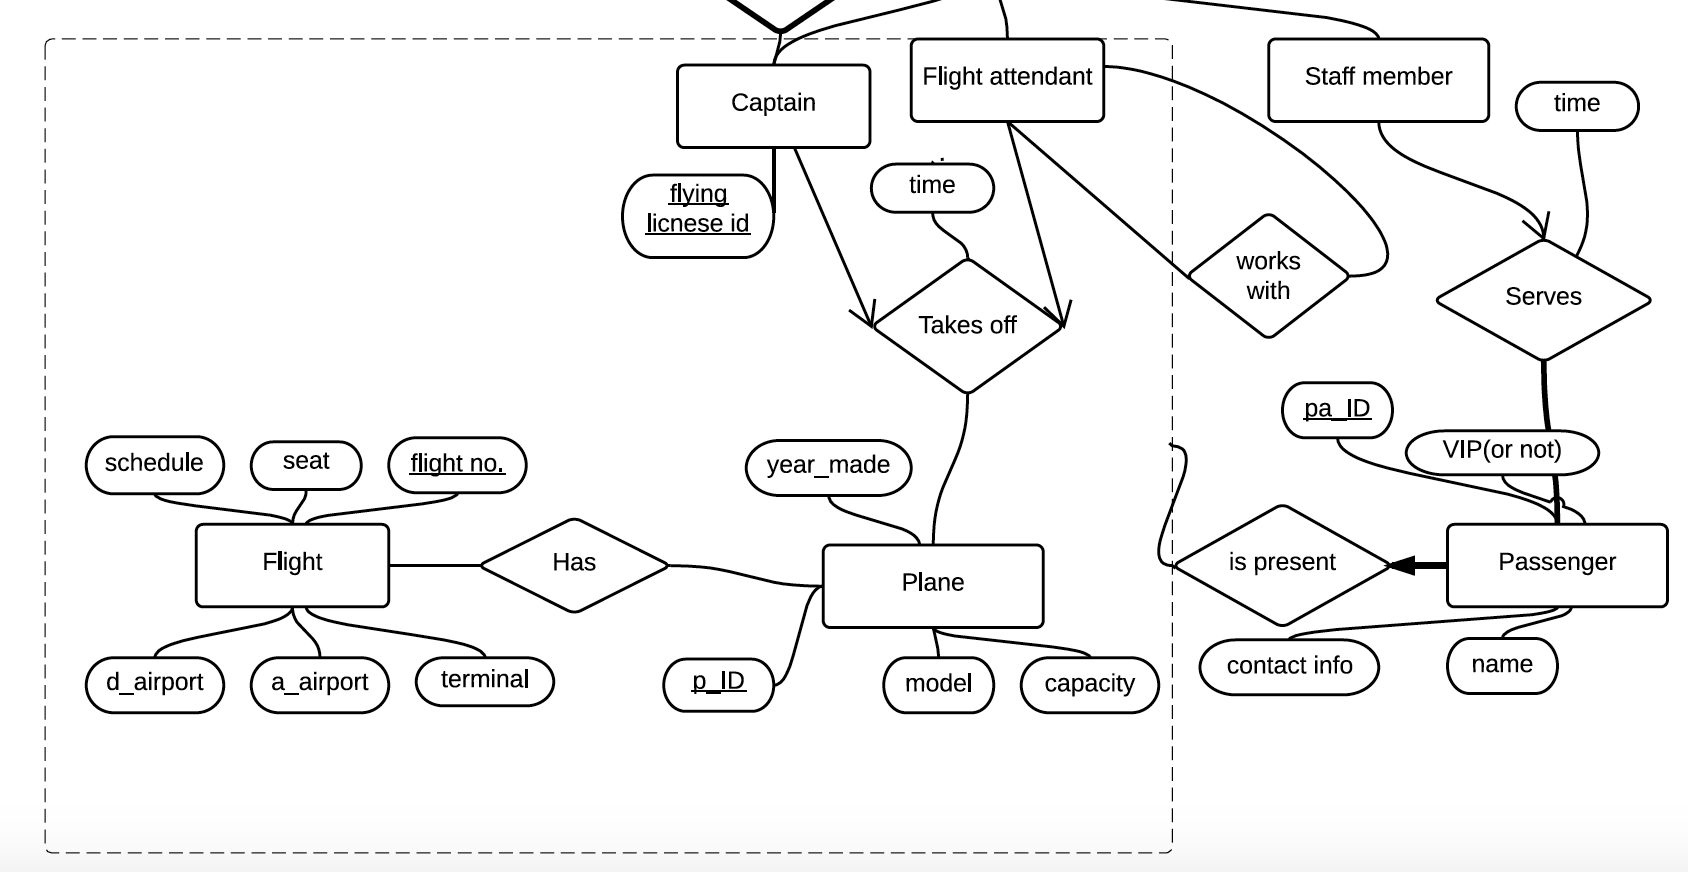
\includegraphics[width=.50\textwidth]{Aggregation.png}
\end{figure}

\vspace{50mm}

\newpage\begin{itemize} \item{
Example of is A- There's a IS-A relation between the four entities captain, flight attendant, staff member and employee. Each employee is a captain or flight attendant or staff member.
Since the subclass inherits the attributes of the superclass, only the superclass has the common attributes that repeat which are the id, name, salary, experience. All the subclasses as well as the superclass will have the same Primary Key (PK). In everyday life, an employee can be either of those entities and can be reached by a passenger or such by their distinguishable attributes and when they are needed.
} \end{itemize} 

\begin{figure}
\centering
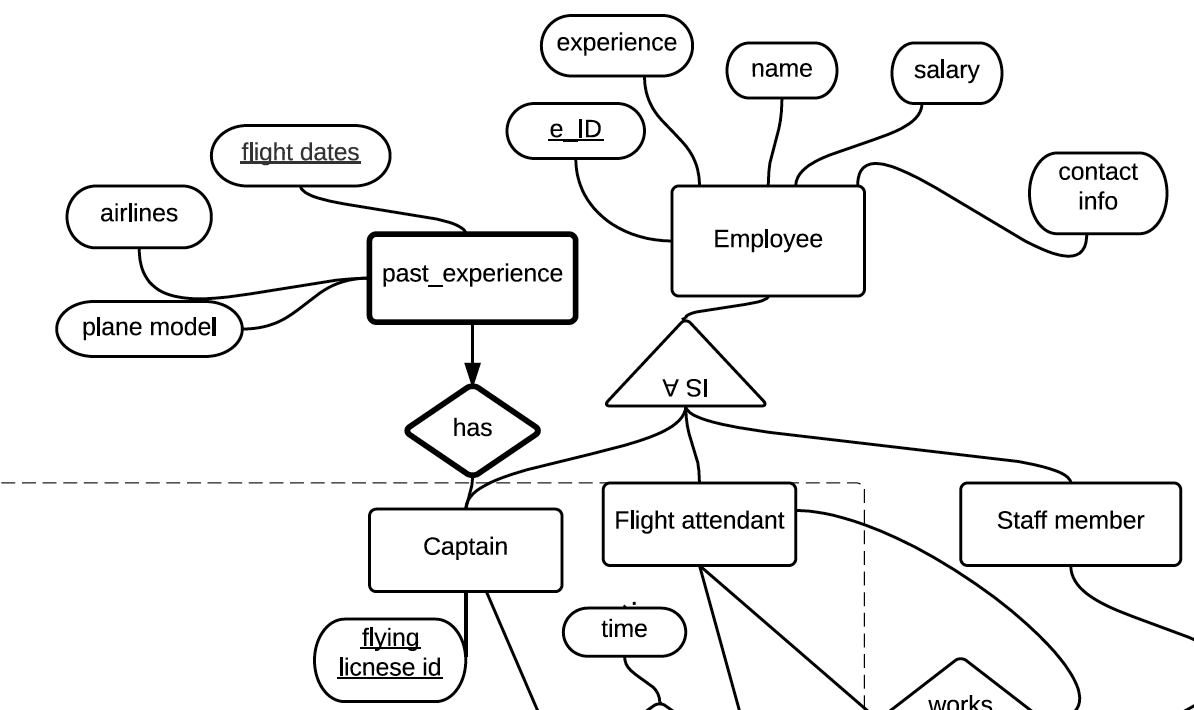
\includegraphics[width=.50\textwidth]{is_a.png}
\end{figure}


\newpage\begin{itemize} \item{
Example of Ternary Relation- The TAKES OFF relation connects three entities: captain, flight and the plane. It is a ternary relation which means that a plane can not take off without a captain and flight attendants.  In everyday life, without a captain, the plane cannot be driven to take off. If a flight attendant is not there to help passengers or something, then the plane cannot take off. If the plane is damaged, it cannot take off. That is why all 3 are needed in order for the plane to take off and it is a ternary.} \end{itemize}

\begin{figure}
\centering
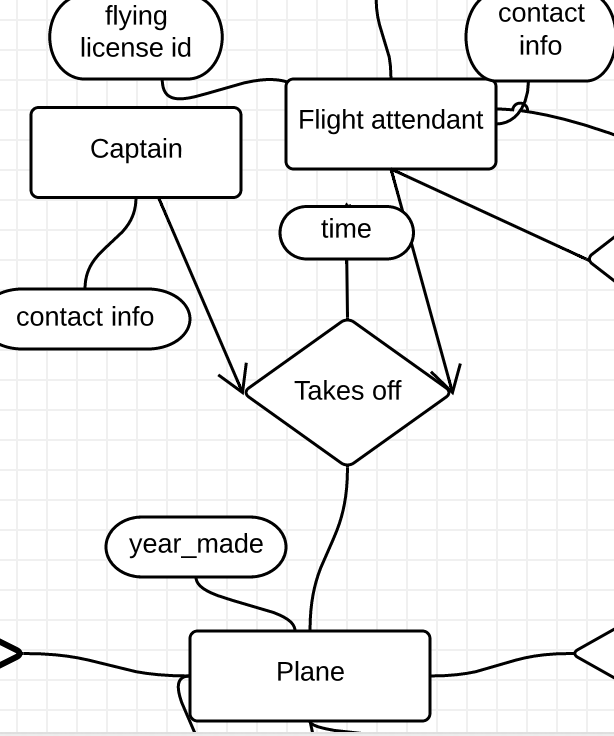
\includegraphics[scale=0.5]{ternary.png}
\end{figure}



\newpage\begin{itemize} \item{
Example of At Most and At Least-  For at least The SERVES relation connects passenger entity and staff member entity. This relation includes an at least constraint and an at most constraint. It can be interpreted as:
Every passenger is served by at least one staff member and every staff member can only serve at most one passenger at a time. In everyday life, one staff member can bring the food to a certain passenger while another can bring drinks. And a staff member giving food can give it to 1 passenger at a time and a staff member can give drinks to 1 passenger at a time.} \end{itemize} 

\begin{figure}
\centering
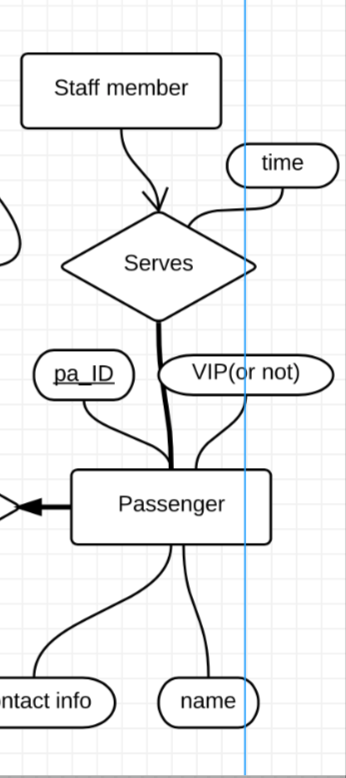
\includegraphics[scale=0.5]{at_most.png}
\end{figure}



\newpage\begin{itemize} \item{
Example of Exactly-  For the is present relation connecting to the passenger entity, it shows that: Each passenger is present on exactly 1 flight. In everyday life, a passenger cannot be on 2 flights at the same time, it's just not possible for an individual to take a trip on 2 of them for 1 flight.} \end{itemize} 

\begin{figure}
\centering
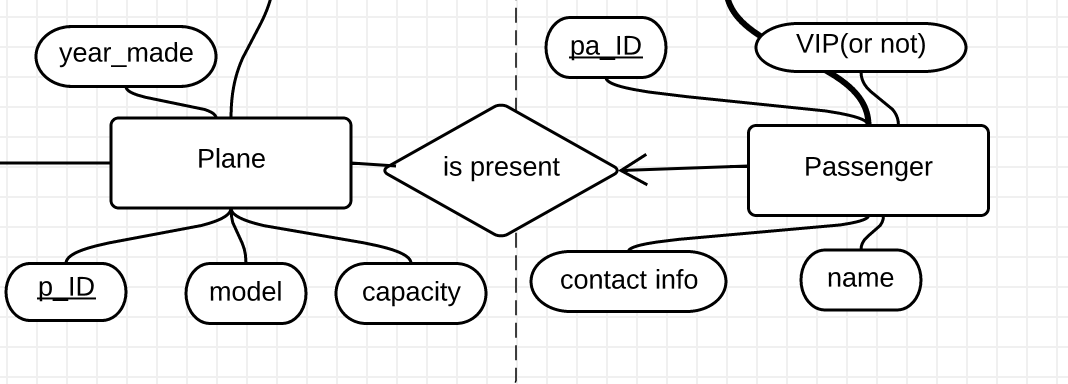
\includegraphics[width=.50\textwidth]{exactlyOne.png}
\end{figure}












\newpage\begin{itemize} \item{
Example of Unary-  Each flight attendant can work with another flight attendant. In everyday life, a attendant might need to team up with another in order to serve passengers faster and more efficiently.} \end{itemize}

\begin{figure}
\centering
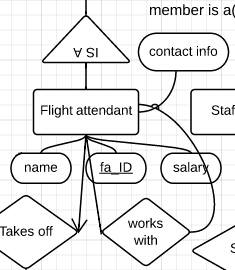
\includegraphics[scale=0.5]{unary.jpg}
\end{figure}


\newpage\begin{itemize} \item{
Example of Weak Entity- The HAS relation connects past experience entity and Captain entity. Here, past experience is a weak entity because if the Captain entity is removed, the instance of pilot past experience is not needed either and taken out. IN everyday life, if a pilot past experience is zero or very low, then a captain would not want to fly on that plane.} \end{itemize}


\begin{figure}
\centering
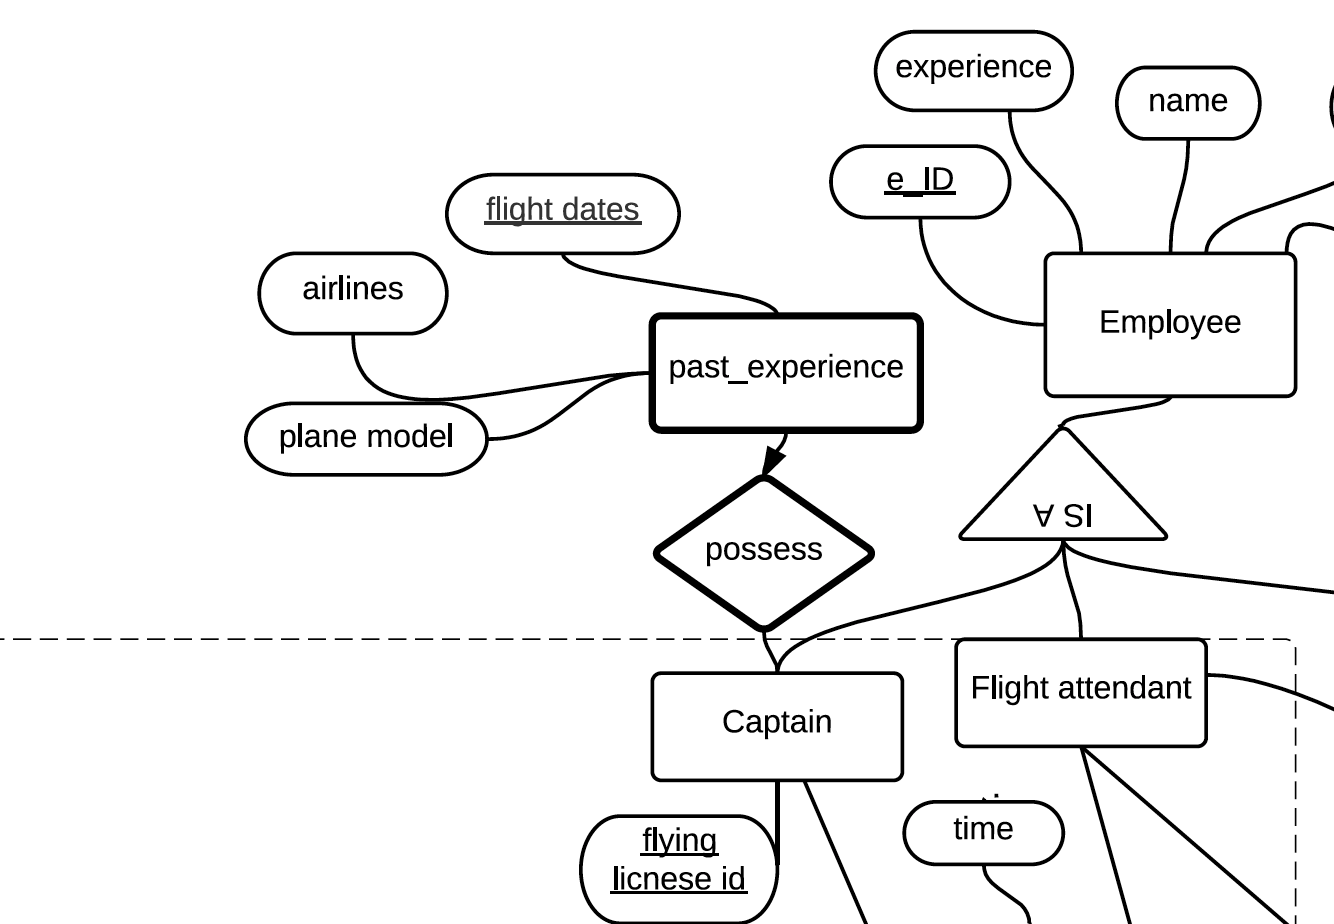
\includegraphics[width=.50\textwidth]{newweak.png}
\end{figure}



\newpage\subsection{Stage3 - The Implementation Stage. }\label{sec: 3 The Implementation Stage.}
%%%%%%%%%%%%%%%%%%%%%%%%%%%%%%%%%%%%%%%%%%%%%%%%%%%%%%%%%%%%%%%%%%%%%%%%%%%%%%%%%%%%%%%%%%%%%%%%%%%%%%%%%%

\begin{itemize} \item{
improvement has taken place to stage2} \end{itemize}


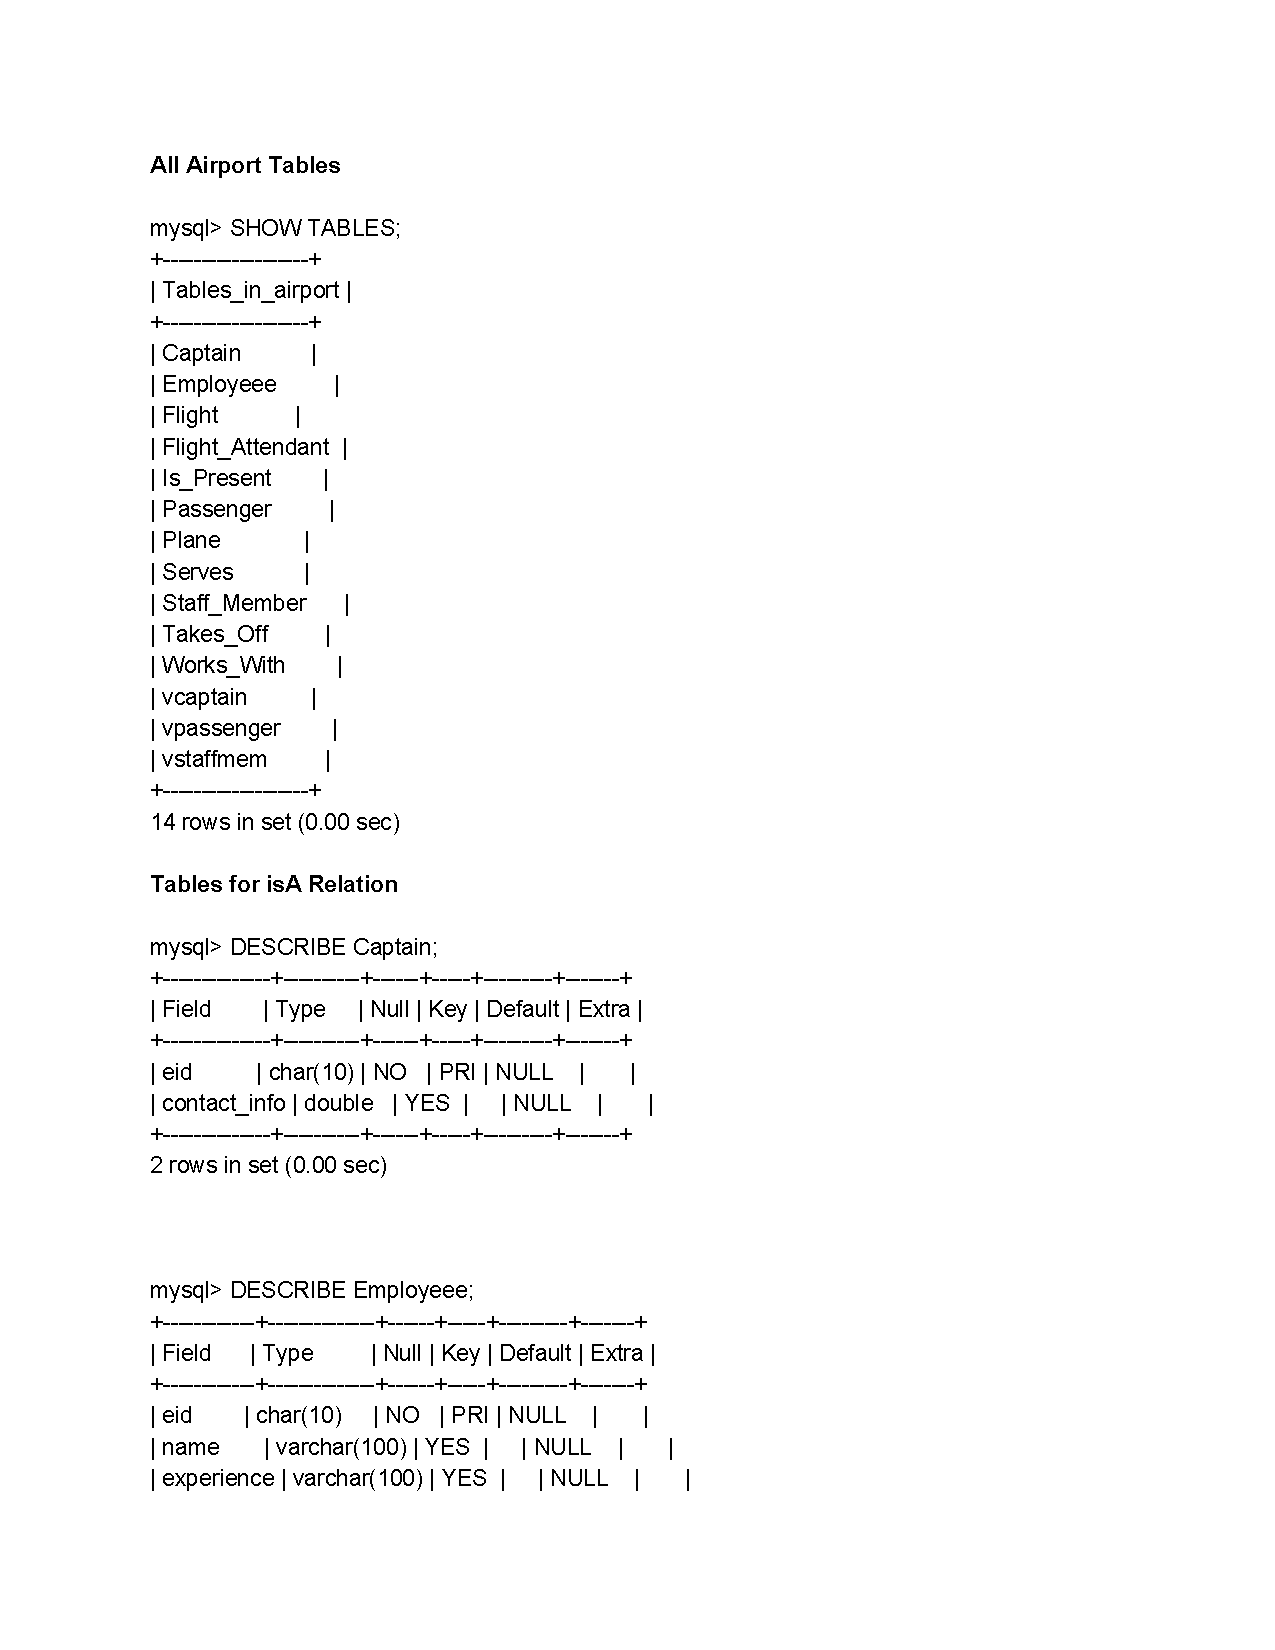
\includepdf[pages=-]{finalsqltables.pdf}

\newpage\begin{itemize} \item{Normalization- Table CAPTAIN is 3NF normalized. It passes 1NF because each row has a primary key which is Employee ID to distinguish it, and no column has one more value saved(like separated with commas). It passes 2NF because contact info attribute depends on Employee ID only. It passes 3NF because there is no transitive dependency in this table. Contact info is the only attribute for captain entity and it depends on eid only.} \end{itemize}

\begin{itemize} \item{Table EMPLOYEE is 3NF-normalized. It passes 1NF because each row has a primary key which is Employee ID to distinguish it, and no column has one more value saved(like separated with commas). It passes 2NF because attributes name, experience and salary depends on Employee ID only. It passes 3NF because there is no partial primary key and transitive dependency in this table.} \end{itemize}

\begin{itemize} \item{Table FLIGHT ATTENDANT is 3NF-normalized. It passes 1NF because each row has a primary key which is Employee ID to distinguish it, and no column has one more value saved(like separated with commas). It passes 2NF because contact info attribute depends on Employee ID only. It passes 3NF because there is no transitive dependency in this table. Contact info is the only attribute for captain entity and it depends on employee ID only.
} \end{itemize}

\begin{itemize} \item{Table STAFF MEMBER is 3NF-normalized. It passes 1NF because each row has a primary key which is Employee ID to distinguish it, and no column has one more value saved(like separated with commas). It passes 2NF because contact info attribute depends on Employee ID only. It passes 3NF because there is no partial primary key and transitive dependency in this table. Contact info is the only attribute for captain entity and it depends on employee ID only.
} \end{itemize}

\begin{itemize} \item{Table PLANE is 3NF-normalized. It passes 1NF because each row has a primary key which is plane ID to distinguish it, and no column has one more value saved(like separated with commas). It passes 2NF because attributes year made, model name and capacity depends on plane ID only. It passes 3NF because there is no partial primary key and transitive dependency in this table.
} \end{itemize}

\begin{itemize} \item{Table PASSENGER is 3NF-normalized. It passes 1NF because each row has a primary key which is Passenger ID to distinguish it, and no column has one more value saved(like separated with commas). It passes 2NF because attributes name, contact info and notVIP depend on passenger ID only. It passes 3NF because there is no partial primary key and transitive dependency in this table.
} \end{itemize}

\begin{itemize} \item{Table WORKS WITH is 3NF-normalized. It passes 1NF because each row has a primary key which is eID and no column has one more value saved (like separated with commas). It passes 2NF because all attributes depend on eID only. It passes 3NF because there is no partial primary key and transitive dependency in this table.
} \end{itemize} 

\begin{itemize} \item{Table TAKES OFF is 3NF-normalized. It passes 1NF because each row has a primary key which is pID and no column has one more value saved (like separated with commas). It passes 2NF because all attributes depend on pID only. It passes 3NF because there is no partial primary key and transitive dependency in this table.
} \end{itemize}

\begin{itemize} \item{Table IS PRESENT is 3NF-normalized. It passes 1NF because each row has primary keys which are paID and pID and no column has one more value saved (like separated with commas). It passes 2NF because all attributes depend on paID and pID only. It passes 3NF because there is no partial primary key and transitive dependency in this table.
} \end{itemize}

\begin{itemize} \item{Table Past Experience is 3NF-normalized. It passes 1NF because each row has primary keys which are flight license id and flightdates and no column has one more value saved (like separated with commas). It passes 2NF because all attributes depend on flight license and flightdates only. It passes 3NF because there is no partial primary key and transitive dependency in this table.
} \end{itemize}

\begin{itemize} \item{Data-Range Constraints - The main data constraints of importance within our database are Flight Attendant, Staff Member, Plane, Passenger, and Flight. For Flight Attendant entity, the contact info must be real numbers and be a phone number. Same applies for flying license id which states their number identification with a real number.} \end{itemize} 

\begin{itemize} \item{For Staff Member entity, the same idea is applied because of having the same fields. The contact info must be real numbers and be a phone number. And their eid must uniquely identify them.} \end{itemize} 

\begin{itemize} \item{For Plane entity, the pid number must uniquely identify them, while the year made must be a date greater than 1990 because we don't want passenger to be on a plane more than 30 years old(the technology has gotten much better since than). And another constraint is the capacity because the max a big plane can hold is about 900.} \end{itemize} 

\begin{itemize} \item{For Passenger entity, the paid number must uniquely identify them, while the contact info phone number can only be a certain amount of bits such as if they are calling an international number. And their flight number cannot be more than 5, because the board which everyone refers to at the airport can only have max 5 numbers on it which identifies the number of the flight.} \end{itemize} 


\begin{itemize} \item{For Flight entity, the seat number can only be 2 bits, the first being a number and the second a letter(e.g 1A, 3B...etc). The terminal can only be 2 bits because up to max 50 to walk to. The flight number is same concept as before for an integer, but the schedule can only be max 2400(this means 12am  Because 24 hours in a day and that identifies the time e.g if it was 2100, it would be 9 o clock...etc). Departure and arrival of airport are just characters that will describe the location. The nonStop entity is 1 bit either y or n, meaning yes or no if the flight is taking a break at a certain destination or not. The status attribute is 10 bits for char either saying on time or delayed.} \end{itemize} 



\begin{itemize} \item{Data Access/Update Constraints - The data access for each user depends on what entities the users need to be able to access to do their job.} \end{itemize} 

\begin{itemize} \item{Flight Attendant and Captains have the same user access. They have access to flight and plane information.They also have access to basic passenger information like seating arrangement and meal information. Flight Attendants do not have access to information about each other.} \end{itemize} 

\begin{itemize} \item{Users that are Passengers only have access to information pertaining to their flight. No other access is granted, as this can present a security risk. A passenger is going to have access to have access to their flight information such as terminal, time of departure and status of flight. They are not given access to plane either, as this would mean giving access to plane model and size, presenting another, albeit minor, security risk.} \end{itemize} 

\begin{itemize} \item{Staff Members have access to all information about passenger and flight. This is all the information regarding the amount of passengers, prices for each seat, seat accommodation, and any other relevant information about the airport and flight that must be given to the passenger. Staff members are given just enough information to facilitate optimal communication between airport, airport employees and passenger.} \end{itemize} 

\begin{itemize} \item{The admin is given access to everything. The admin has access to every aspect of the database and this works best if the admin also work with the main supervisor of the airport, to make sure that all changes the admin makes are correct. } \end{itemize} 

\newpage\subsection{Stage4 -	User Interface. }\label{sec: 4.	User Interface.}
%%%%%%%%%%%%%%%%%%%%%%%%%%%%%%%%%%%%%%%%%%%%%%%%%%%%%%%%%%%%%%%%%%%%%%%%%%%%%%%%%%%%%%%%%%%%%%%%%%%%%%%%%%

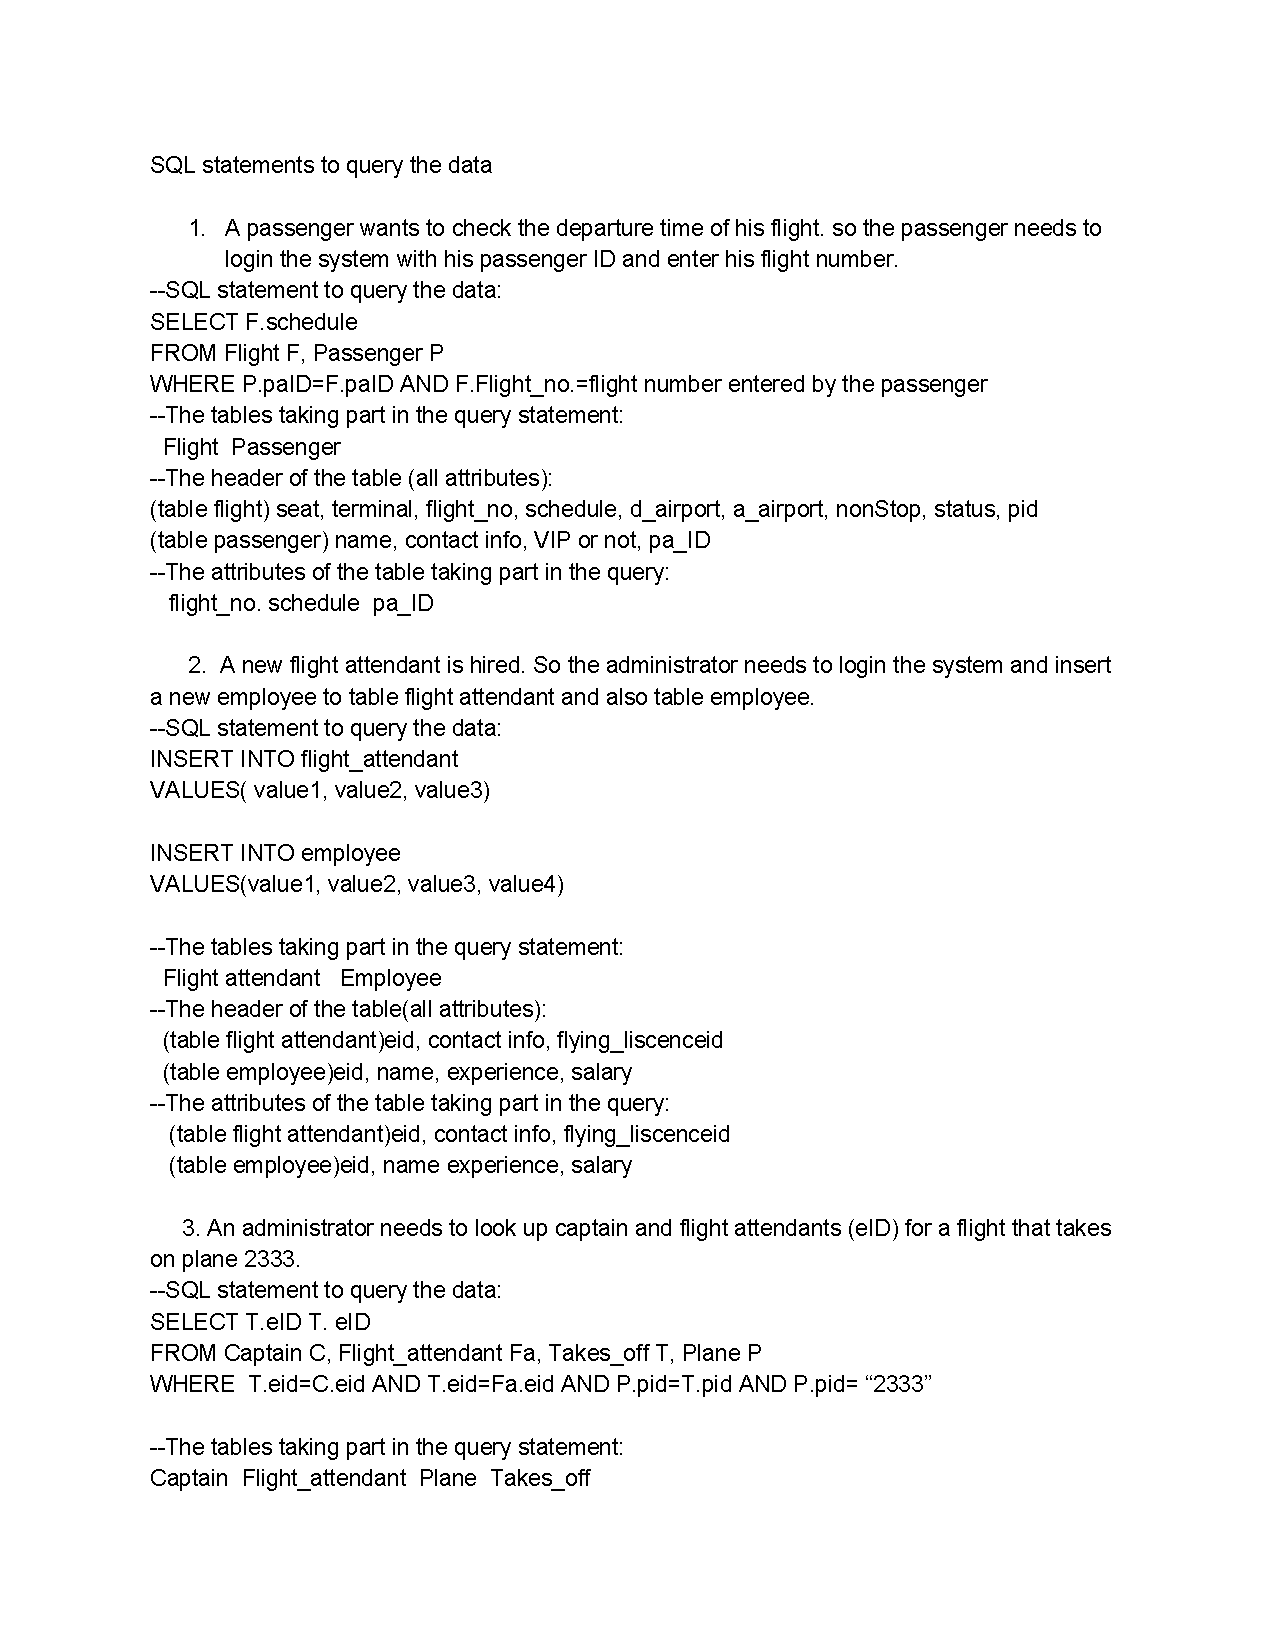
\includepdf[pages=-]{stage4sqlstatements.pdf}

\begin{itemize} \item{1.Error messages that would pop-up when users access and/or updates are denied.
First, Captains and Flight-Attendants have access to flight, plane, and basic passenger information. However, if a flight-attendant tries to access another flight-attendant's information, it will come up as "error- cannot access this information".} \end{itemize}

\begin{itemize} \item{Second, passengers only have access to information about their flight. Because of security, they can only see their own info. If they try to access other peoples info like the captain, they will see a window pop up saying "error-access denied"} \end{itemize}

\begin{itemize} \item{Third, staff members can access information about passenger and flight such the amount of passengers, seat accommodation, prices for each seat, pretty much any information needed to accommodate the passengers to the best of their ability. If any other information is accessed that is not included in this list, an error will pop up saying "error-access denied."} \end{itemize}

\begin{itemize} \item{Fourth, the admin has access to all the aspects of the database and so no errors will pop up for them.} \end{itemize}



\begin{itemize} \item{2.Error messages corresponding to the integrity constraints- First, for the at least integrity constraint, every staff member serves at least one passenger; if a staff member serves no passengers and one is waiting, then an error should pop up "error- flight attendant must assist a passenger waiting" and basically help at least one passenger.} \end{itemize}

\begin{itemize} \item{Second, for the at most integrity constraint, a flight attendant can work on at most one flight at one time; it just doesn't work if an attendant is assigned to 2 flights and if this happens, an error should pop up saying "error- attendant cannot be assigned to 2 different flights."} \end{itemize}


\begin{itemize} \item{Third, for the exactly integrity constraint, one flight can only be on exactly one plane; it just doesn't work if a flight is assigned to 2 planes and if this happens, an error should pop up saying "error- 1 flight assigned to 1 plane, cannot be assigned to 2 different planes."} \end{itemize}

\begin{itemize} \item{The Integrity Constraints are related to the admin view. The ability to add or take out an instances from an table depend on what is the primary key and foreign for that table and all the entities involved. The Flight table has a primary key, which is fid. It also has a foreign key, which is pid of the plane. This means that when the admin adds a new instance as a tuple into the flight table, the admin must include a primary and foreign key.
} \end{itemize}


\begin{itemize} \item{The error messages corresponding to the data range constraints violations.} \end{itemize}

\begin{itemize} \item{First, for flight attendant, the input has to be a real number and thus the phone number and contact info will be. Otherwise, if the id is not a real, it will pop up as an error.} \end{itemize}

\begin{itemize} \item{Second, for staff member, the same idea for errors popping up is applied. The id must be real and thus the contact info..etc should be.} \end{itemize}

\begin{itemize} \item{Third, for Plane, if a date for a plane is not 1990 or greater for a plane made, an error will come up. If the capacity for a plane is already 900 and a staff member is trying to board a passenger onto the plane, it will pop up as an error saying "error- plane capacity is full, must board another flight."} \end{itemize}

\begin{itemize} \item{Fourth, for passenger, the error window would come up if the contact info is longer than a certain amount of bits(if the number is longer than an international call). If the flight number is more than 5, an error message would come up saying "error-number flight number must be 5 or lower.} \end{itemize}

\begin{itemize} \item{Fifth, for Flight, if the seat number is more than 2 bits, then an error window would pop up saying "error-seat number must be 2 bits(the first being a number and the second being a letter)." If the terminal is more or less than 2 bits and greater than 50, then an error window would pop up saying "error- only terminals 1-50. The flight number is the same concept as before for an integer, but the schedule can only be max 2400 for 12:00am, otherwise an error would say "error- not a real time." The arrival and departure are just characters describing the location, if characters not entered, then "error- enter location again." The nonstop entity is either a y or n for yes or no, otherwise anything else entered would be a error and it would read "error- enter either y or n."} \end{itemize}

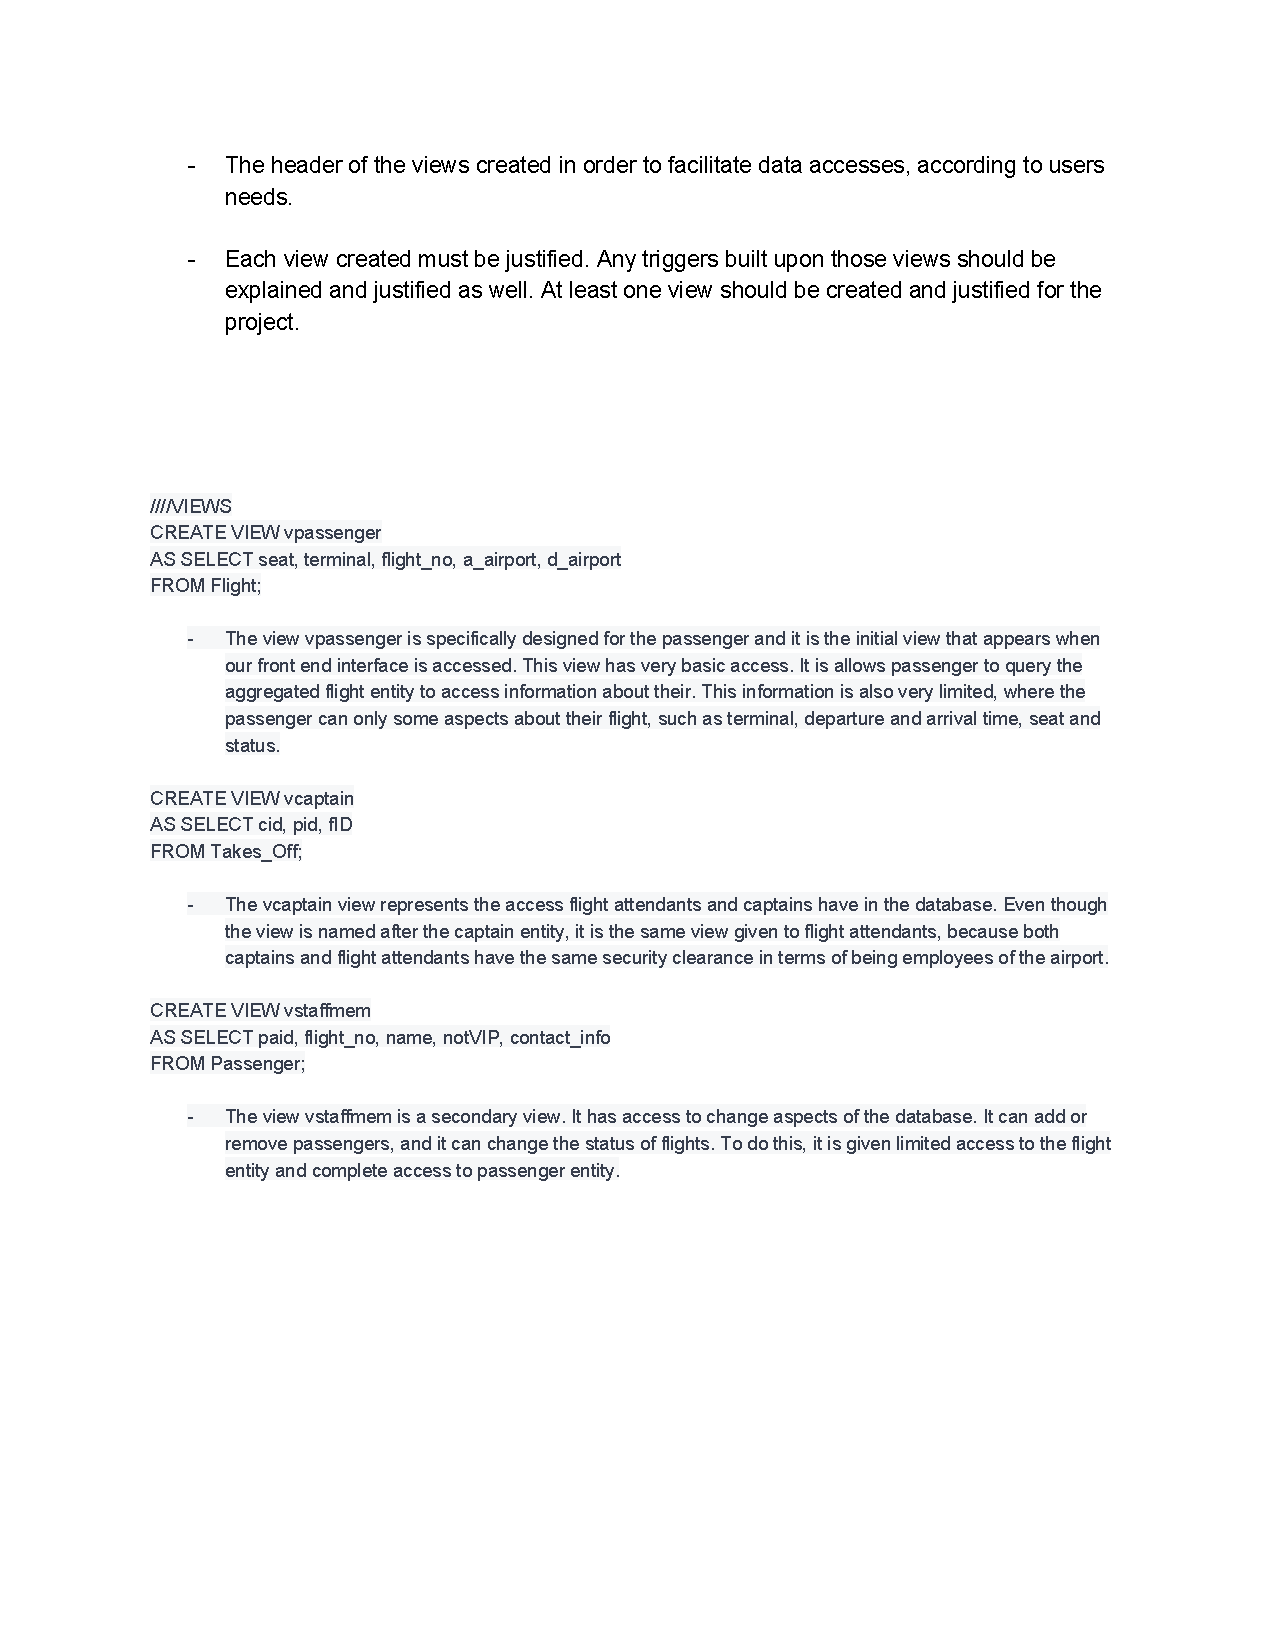
\includepdf[pages=-]{views.pdf}




\section{END}\label{sec:7. Project Highlights.}
%%%%%%%%%%%%%%%%%%%%%%%%%%%%%%%%%%%%%%%%%%%%%%%%%%%%%%%%%%%%%%%%%%%%%%%%%%%%%%%%%%%%%%%%%%%%%%%%%%%%%%%%%%



\bibliographystyle{IEEEtran}
%\bibliography{IEEEabrv,bib_queyroi_abello2013}
%\bibliography{bib_queyroi_abello2013}

\end{document}